\graphicspath{{img/intro/out}}


\chapter{Introduction}
\label{ch:intro}

\section{Artificial Intelligence}
\label{sec:artificial-intelligence}
Artificial Intelligence (AI) is a broad subject of study that can be defined in different ways~\cite[chapter 1]{russell_artificial_2021}.
John McCarthy, often called the “father of AI”~\cite{wiki_ai_2023, woo_fatherofai_2014, andresen_fatherofai_2002}, defines it as “the science and engineering of making intelligent machines”~\cite{stanford-whatisai}, where intelligence means “the computational part of the ability to achieve goals in the world”~\cite{stanford-whatisai}.
AI is sometimes mistakenly used interchangeably with Machine Learning.
Machine learning is a subset of AI concerned with enabling AI systems to learn from experience~\cite[chapter 1]{russell_artificial_2021}.
Machine learning enables the development of large-scale AI systems as they are used today.
\\
The study of artificial intelligence was first proposed by McCarthy et al. in late 1955 \cite{mccarthy_proposal_1955}.
It went through two major hype cycles in the sixties and the eighties~\cite{googlengram_ai, wiki_ai_2023, sitnflash_history_2017} followed by phases of “AI winter”.
The current (as of early 2024) AI boom, sometimes also called “AI spring”~\cite{aispring} was started by groundbreaking advances in speech recognition~\cite{hinton_deep_2012} and image classification~\cite{krizhevsky_imagenet_2012} in 2012~\cite{google_decade_2021, house_2012_2019} and reached the public at the latest in late 2022, following the release of ChatGPT~\cite{openai_chatgpt_intro}, a multipurpose AI-chatbot, open to everyone~\cite{openai_chatgpt}.
\\
These breakthroughs are made possible mainly by advancements in the field of machine learning, enabling AI systems to learn from huge amounts of data.
In addition, the exponential increase in computation and storage capabilities as predicted by Moore’s Law~\cite{mooreslaw}, algorithms like backpropagation~\cite{rumelhart_learning_1986} allowed incorporating large amounts of data into machine learning models in realistic amounts of time.
\\
Today, AI systems are indispensable in many areas such as web search engines~\cite{google_howweuseai}, recommendation systems~\cite{burke_recommender_2011}, human speech recognition and generation~\cite{elevenlabs, hinton_deep_2012}, image recognition and generation~\cite{midjourney, krizhevsky_imagenet_2012} and personal assistants~\cite{openai_chatgpt_intro} and surpasses humans in high level strategy games like go and chess~\cite{silver_mastering_2016, silver_mastering_2017} as well as other video games~\cite{piper_ai_2019}.

\chapter{Neural Networks}
\label{ch:neural-networks}
\section{Overview}
\label{sec:overview}
At the heart of almost all the technologies mentioned in the last paragraph are deep artificial neural networks.
The next section will outline the mathematical details of how these systems work and learn.
Although the comparison of artificial neural networks, from now on just called “neural networks”, to their biological counterpart can be criticized as oversimplifying the inner workings of biological brains~\cite[chapter 1.1]{aggarwal_neural_2018}, the architecture of neural networks is heavily inspired by how decision-making and learning work in the human brain~\cite[chapter 1.1]{aggarwal_neural_2018, mit_nnexplained}.
I will illustrate the basic principles of neural networks at the example of a network that detects the gender of a person by looking at pictures.
\\
\\
A neural network consists of a number of layers of artificial neurons, called \textit{nodes}.
In a \textit{fully connected} network, each node is connected to every node in the next layer.
The connection strengths are called \textit{weights}.
An image of a person can be fed into the network by setting the \textit{activation} values of the first layer of the network, the \textit{input layer}, to the individual pixel values of the image.
This information is then fed forward through the layers of the network until the \textit{output layer} is reached.
If a network has at least one layer in between the input and output layer, it is called a \textit{deep neural network}.
These intermediate layers are called \textit{hidden layers}.
If the outputs of each layer are only connected to the inputs of the next layer, the network is called a \textit{feedforward neural network}.
If \textit{feedback} connections are allowed, the network is called a \textit{recurrent neural network}.
\\
In our example, the output layer should consist of only two nodes.
If the activation of the first node is larger than the activation of the second node, the network thinks that the person in the picture is a male.
If on the other hand the second node has a larger activation, the network classifies this person as female~\cite[chapter 1.2]{aggarwal_neural_2018}.
\\
\\
In order to make accurate predictions, a reasonable set of network parameters (i.e.the weights) has to be found.
This is done by training the network with pre-classified images.
After an image has been processed by the network, the output is compared to the correct classification and the network parameters are updated in a way that would improve the networks output if the same image was to be processed again~\cite[chapter 1.2]{aggarwal_neural_2018,ibm_nn}.
\\
This is similar to how humans learn from experience.
If we were to misclassify a persons gender, the unpleasant social experience that may come with that mistake would cause us to update our internal model of what different genders look like to not make the same mistake again.
\\
\\
One of the main strengths of neural networks is their ability to \textit{generalize}~\cite{gonfalonieri_understand_2020}.
When a network was trained on a large enough set of examples, it gains the ability to generalize this knowledge to examples that were previously unseen.
The gender classification network from our example doesn't just memorize the genders of the people it has seen, but instead learns about the features that help to identify the gender of a random person.
\\
\\
The problem of image classification is a rather complex one.
One wouldn't typically think of it as finding a function that maps the values of each input pixel to the classification output.
But even very complex problems can be modeled by equally complex functions.
The universal approximation theorem states, that a feedforward neural network with at least one hidden layer with appropriate activation functions (see~\ref{subsec:activation-functions} for details) can approximate any continuous function if given enough nodes~\cite[chapter 6.4.1]{goodfellow_deep_2016}.
That's why training a neural network can be thought of as fitting the network to the training data.
\\
\section{Mathematical Details}
\label{sec:nn-mathematical-details}
The following section will outline the mathematical details of how neural networks work.
The definitions and derivations are based on~\cite[chapter 1.2-1.3]{aggarwal_neural_2018},~\cite[chapter 5-6]{goodfellow_deep_2016},~\cite{ibm_nn} as well as~\cite[chapter 4.4]{haykin_neural_1998}.
\\
\\
The most complete treatment of the mathematical details of neural networks is arguably given by the framework of computational graphs~\cite{bettilyon_computationalgraphs_2020}.
In this framework, a neural network is treated as single that maps a set of input values to a set of output values.
This function is composed of individual mathematical operations and can be represented as a directed graph \cite[section 1.4]{haykin_neural_1998}.
I will not rigorously define the framework of computational graphs here, as this is beyond the scope of this thesis.
Instead, I will explain the principles of neural networks starting from a single neuron and then build up to a fully connected neural network. 
\subsection{Notation}
\label{subsec:nn-notation}
The following notation will be used throughout this section:
\begin{equation*}
    \begin{array}{ll}
    \bm{x} & : \text { input vector of the neural network} \\
    \bm{a} & : \text { activation vector of a layer} \\
    \bm{z} & : \text { pre-activation vector of a layer} \\
    \bm{y} & : \text { output vector of the neural network} \\
    \bm{b} & : \text { bias vector of a layer} \\
    x_i, a_i, z_i, y_i, b_i & : \text { individual elements of the respective vectors, for individual nodes } \\
    \bm{w_i} & : \text { weight vector of all weights connected to neuron i} \\
    w_{ij} & : \text { weight of the connection from neuron i of a layer to neuron j of the previous layer } \\
    W & : \text { weight matrix of a layer. Contains rows $\bm{w_i}$} \\
    ^{[J]} & : \text { superscript denoting the layer of a variable} \\
    \end{array}
\end{equation*}
\subsection{Single Node}
\label{subsec:single-neuron}
\begin{figure}
    \centering
    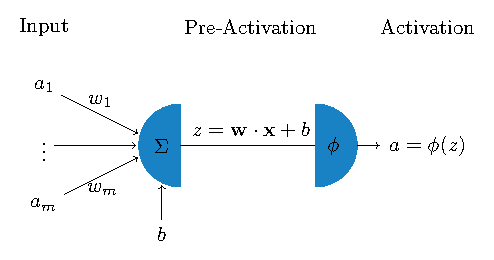
\includegraphics[width=0.5\textwidth]{single_neuron}
    \caption{A single node of a neural network. To get the activation $a$ of the node, the pre-activation $z$ is calculated from the inputs $a_i$ and the bias $b$ and is passed through an activation function $\phi$.}
    \label{fig:single-neuron}
\end{figure}
Before we can build a neural network out of nodes, we have to define how a single node works.
Each node receives the activations $a_i$ from the nodes of the previous layer as inputs. 
Each connection is assigned a weight $w_i$, stored in the node's weight vector $\bm{w}$.
\\
Additionally, each node has a so-called \textit{bias} $b$. 
The bias shifts the net input of the node by a constant value.
It is needed to model certain problems where part of the prediction is independent of the input \cite[6]{aggarwal_neural_2018}.
Examples include all problems where the output should not be zero even if all inputs are zero. 
\\
\\
The net input, called \textit{pre-activation value} $z$ of a node is the weighted sum of all inputs plus the bias:
\begin{equation}
    z = \sum_{i=1}^{m} w_i a_i + b = \bm{w} \cdot \bm{a} + b \text{.}
    \label{eq:pre-activation}
\end{equation}
The pre-activation value is then passed through an \textit{activation function} $\phi$ to get the activation $a$ of the node, which is then passed on to the next layer, where the process is repeated:
\begin{equation}
    a = \phi(z) \text{.}
    \label{eq:activation}
\end{equation}
The whole process is illustrated in figure \ref{fig:single-neuron}.

\subsection{Activation Functions}
\label{subsec:activation-functions}
The activation function $\phi$ is used to introduce non-linearity into the network and thus increasing its modeling power \cite[section 1.2.1.3]{aggarwal_neural_2018}. 
Some activation functions are also referred to as \textit{squashing function}~\cite[10]{haykin_neural_1998}, as they map the unbounded pre-activation value $z$ to a bounded activation value $a$.
The choice of activation function has a large impact on the performance of the network in terms of both accuracy and speed \cite{dubey_activation_2022}.
The type of function heavily influences the way that information is processed by the network and the complexity of the function naturally has a large impact on the computational cost of the network.
The best choice therefore depends on the problem that is being solved and the architecture of the network.
Typically, the same activation function is used for all nodes in a layer and is applied to the pre-activation value of each node individually, but different layers can use different activation functions depending on their purpose \cite[174]{goodfellow_deep_2016}.
For a long time, the most popular activation functions were (\cite[chapter 6.3]{goodfellow_deep_2016}, \cite[section 1.2.1.3]{aggarwal_neural_2018}) the sigmoid function:
\begin{equation}
    \phi(z) = \sigma(z) = \frac{1}{1+e^{-z}}
    \label{eq:sigmoid}
\end{equation}
and the hyperbolic tangent function:
\begin{equation}
    \phi(z) = \tanh(z) = \frac{e^z - e^{-z}}{e^z + e^{-z}} = 2\sigma(2z) - 1
    \label{eq:tanh}
\end{equation}
as well as the sign function:
\begin{equation}
    \phi(z) = \text{sign}(z) = \begin{cases}
        1 & \text{if } z > 0 \\
        0 & \text{if } z = 0 \\
        -1 & \text{if } z < 0 \text{.}
    \end{cases}
    \label{eq:sign}
\end{equation}
The sign function can map neural network output to a binary classification, but it is not suitable for backpropagation (see section \ref{subsec:backprop}) due to its derivative being zero almost everywhere.
The sigmoid function and the hyperbolic tangent function are both differentiable and limit the output to the range $(-1, 1)$ and $(0, 1)$ respectively.
They are however more computationally expensive than other activation functions and suffer from the \textit{vanishing gradient problem}.
The vanishing gradient problem is caused by the fact that the derivative of the sigmoid function approaches zero for large absolute values of $z$.
This leads to the weights of the nodes in the first layers of the network being updated very slowly, as the gradient of the loss function with respect to the weights of these nodes is very small (see section \ref{subsec:backprop})\cite[section 1.4.2]{aggarwal_neural_2018}\cite{dubey_activation_2022}.
The sigmoid function and the hyperbolic tangent function can be seen in figure \ref{fig:sigmoid} and \ref{fig:tanh}.
\begin{figure}
    \centering
    \begin{subfigure}[b]{0.45\textwidth}
        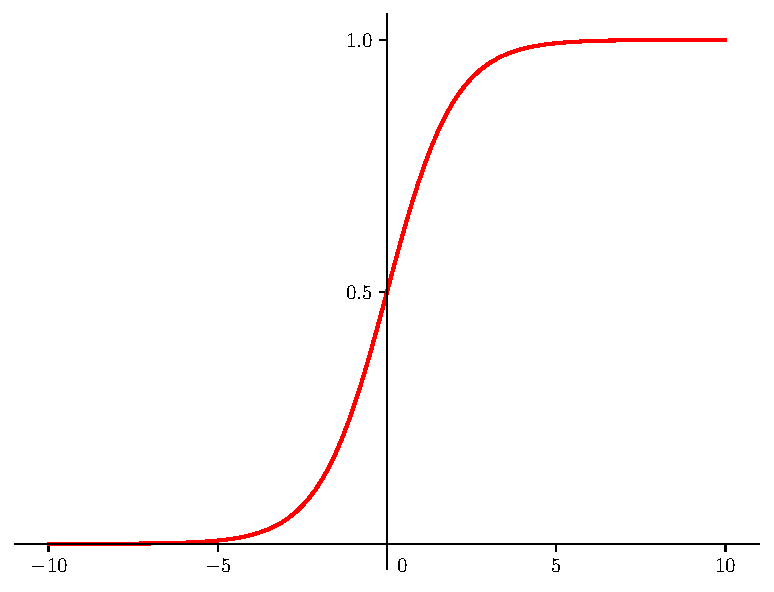
\includegraphics[width=\textwidth]{sigmoid}
        \caption{The sigmoid activation function.}
        \label{fig:sigmoid}
    \end{subfigure}
    \hfill
    \begin{subfigure}[b]{0.45\textwidth}
        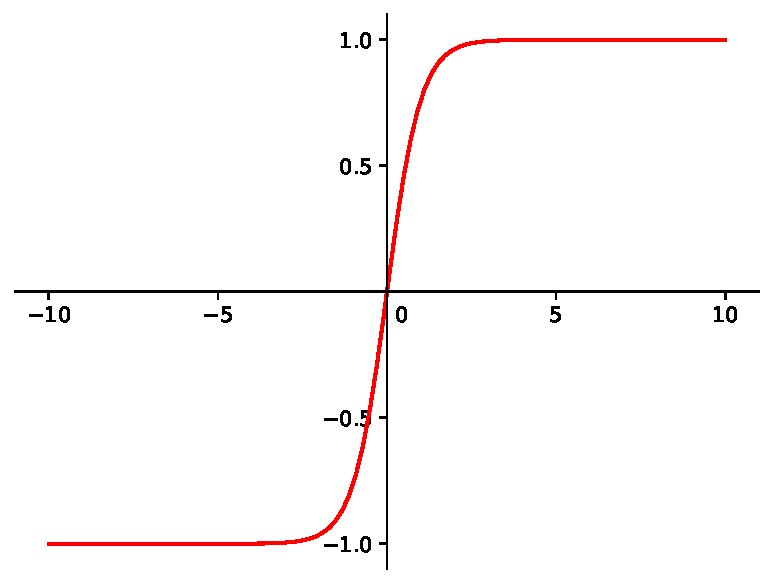
\includegraphics[width=\textwidth]{tanh}
        \caption{The hyperbolic tangent activation function.}
        \label{fig:tanh}
    \end{subfigure}
    \caption{The most popular activation functions before the rise of ReLU.}
    \label{fig:tanhsigmoid}
\end{figure}
\\
\\
In recent years, the \textit{rectified linear unit} (ReLU) and similar stepwise linear functions have become the go-to activation functions for deep neural networks~\cite[chapter 6.3.2]{goodfellow_deep_2016}\cite{dubey_activation_2022}.
ReLU is defined as:
\begin{equation}
    \phi(z) = \max(0, z) = \begin{cases}
        0 & \text{if } z \leq 0 \\
        z & \text{if } z > 0 \text{.}
    \end{cases}
    \label{eq:relu}
\end{equation}
Its main advantage is its very low computational cost, as it consists of only a single comparison. 
Although it is not as prone to the vanishing gradient problem as the sigmoid and the hyperbolic tangent, the problem still exists for negative values of $z$. 
This has been addressed by variations like \textit{Leaky ReLU}, introducing a small but non-zero slope for negative values~\cite{dubey_activation_2022}:
\begin{equation}
    \phi(z) = \max(0.01 z, z) = \begin{cases}
        0.01 z & \text{if } z \leq 0 \\
        z & \text{if } z > 0 \text{.}
    \end{cases}
    \label{eq:leaky-relu}
\end{equation}
The ReLU function and its leaky version can be seen in figures \ref{fig:relu} and \ref{fig:leaky-relu}.
\begin{figure}
    \centering
    \begin{subfigure}[b]{0.45\textwidth}
        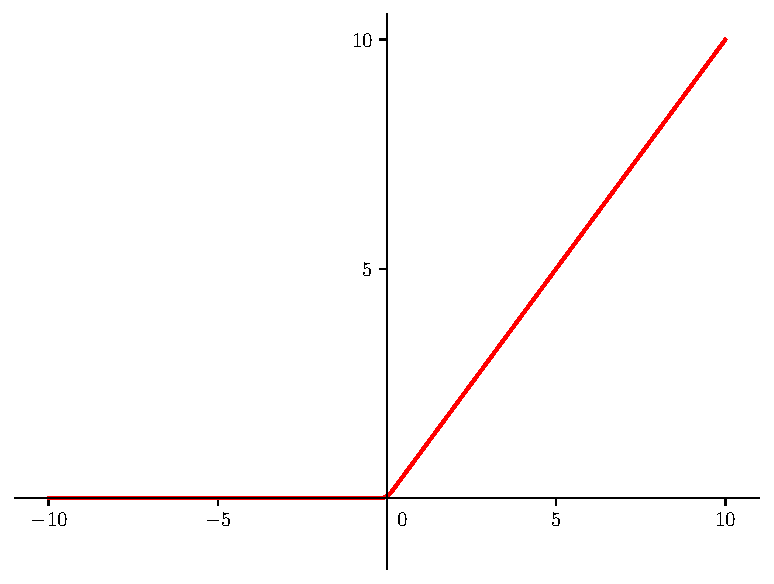
\includegraphics[width=\textwidth]{relu}
        \caption{The rectified linear unit (ReLU) activation function.}
        \label{fig:relu}
    \end{subfigure}
    \hfill
    \begin{subfigure}[b]{0.45\textwidth}
        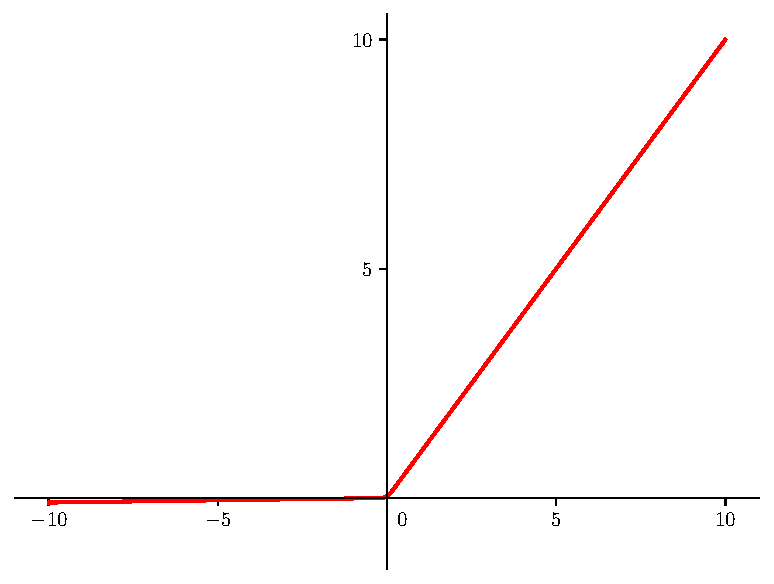
\includegraphics[width=\textwidth]{leaky_relu.pdf}
        \caption{The leaky rectified linear unit (Leaky ReLU) activation function.}
        \label{fig:leaky-relu}
    \end{subfigure}
    
    \caption{Modern, stepwise linear activation functions.}
    \label{fig:subfigures}
\end{figure}


\subsection{Forward-Propagation in Feedforward Neural Networks}
\label{subsec:forward-propagation}
\begin{figure}
    \centering
    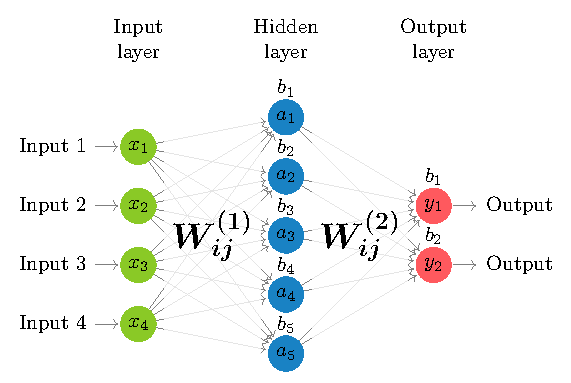
\includegraphics[width=0.9\textwidth]{nn}
    \caption{A feedforward neural network with one hidden layer.}
    \label{fig:nn}
\end{figure}
Now that the workings of the nodes are defined, we can build a fully connected neural network out of these building blocks. 
I will illustrate the process at the example of a feedforward neural network as defined in section \ref{sec:overview}.
An example of such a network can be seen in figure \ref{fig:nn}. 
\\
\\
The process of feeding an input vector $\bm{x}$ through the network to get the output vector $\bm{y}$ is called \textit{forward-propagation}, as the information propagates through the network layer by layer. The activation of any layer $\bm{a}^{[J]}$ can be calculated from the activation of the previous layer $\bm{a}^{[J-1]}$ by generalizing equation \ref{eq:pre-activation} and \ref{eq:activation} to the vector case:
\begin{equation}
    z_k^{[J]} = \sum_{i=1}^{m} w_{ki}^{[J]} a_i^{[J-1]} + b_k^{[J]} \implies \bm{z}^{[J]} = W^{[J]} \bm{a}^{[J-1]} + \bm{b}^{[J]} \text{,}
    \label{eq:pre-activation-vector}
\end{equation}
\begin{equation}
    a_k^{[J]} = \phi(z_k^{[J]}) \implies \bm{a}^{[J]} = \phi(\bm{z}^{[J]}) \text{,}
    \label{eq:activation-vector}
\end{equation}
where the activation function $\phi: \mathbb{R}^m \rightarrow \mathbb{R}^m$ is applied element-wise.
The activation of the input layer $\bm{a}^{[0]}$ is simply the input vector $\bm{x}$ and the activation of the output layer $\bm{a}^{[L]}$ is the output vector $\bm{y}$.
\\
\\
Equations \ref{eq:pre-activation-vector} and \ref{eq:activation-vector} can be applied recursively to calculate the activation of each layer from the input layer to the output layer:
\begin{align}
    \bm{y} = \bm{a}^{[L]} &= \phi(W^{[L]} \bm{a}^{[L-1]} + \bm{b}^{[L]}) \\
    &= \phi(W^{[L]} \phi(W^{[L-1]} \bm{a}^{[L-2]} + \bm{b}^{[L-1]}) + \bm{b}^{[L]}) \\
    &= \phi(W^{[L]} \phi(W^{[L-1]} \phi(\dots \phi(W^{[1]} \bm{x} + \bm{b}^{[1]}) \dots) + \bm{b}^{[L-1]}) + \bm{b}^{[L]}) \text{.}
    \label{eq:forward-propagation}
\end{align}
This equation also shows the significance of the activation function. 
Without it, the whole network would be equivalent to a single layer and could be replaced by a single matrix multiplication.
It would therefore only be able to model linear functions. 
To show this, let's set $\phi(z)$ to the identity in equation \ref{eq:forward-propagation}. This yields:
\begin{align}
    \bm{y} &= W^{[L]} W^{[L-1]} \dots W^{[1]} \bm{x} + \bm{b}^{[L]} + W^{[L]} \bm{b}^{[L-1]} + \dots + W^{[L]} W^{[L-1]} \dots W^{[2]} \bm{b}^{[1]} \\
    &= \widetilde{W} \bm{x} + \tilde{\bm{b}} \text{.}
    \label{eq:linear-network}
\end{align}

\subsection{Loss Functions and Gradient Descent}
\label{subsec:loss-functions}
In order to produce meaningful output, the network's weights and biases have to be adjusted to minimize the error of the network's output.
This process is called \textit{training} the network.
The error of the network is measured by a \textit{loss function} $\lambda(\bm{y}, \bm{\hat{y}})$, where $\bm{\hat{y}}$ is some target output vector.
The loss function is a measure of how far the network's output $\bm{y}$ is from the target output $\bm{\hat{y}}$.
As we want to minimize the network's error, the training process is essentially an optimization problem \cite[chapter 4.3]{goodfellow_deep_2016}.
Let's step back from neural networks for a moment and look at a method to minimize a function $f(\bm{x})$ with respect to its parameters $\bm{x}$.
The most common method to do this in machine learning is \textit{gradient descent} \cite[chapter 4.3]{goodfellow_deep_2016}.
\\
\\
\begin{figure}
    \centering
    \begin{subfigure}[b]{0.45\textwidth}
        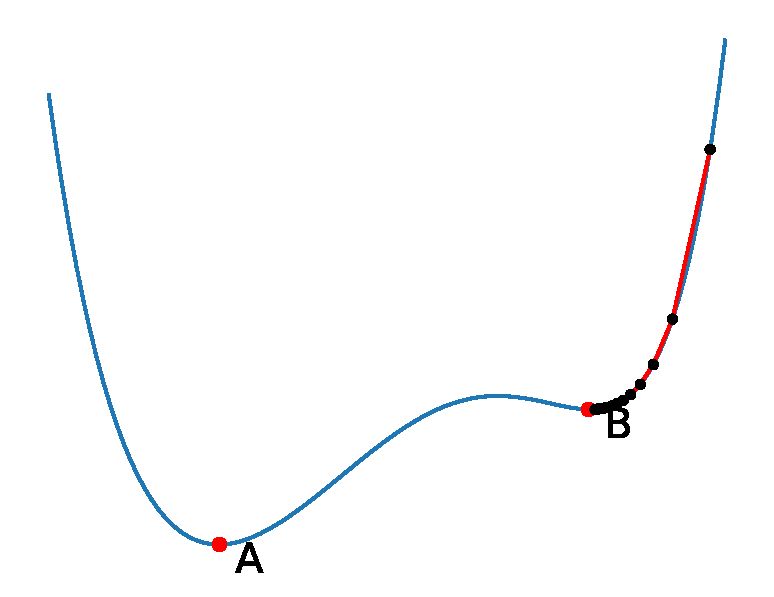
\includegraphics[width=\textwidth]{gradient_descent_small_lr}
        \caption{Gradient descent with a small learning rate.}
        \label{fig:gradient-descent-small}
    \end{subfigure}
    \hfill
    \begin{subfigure}[b]{0.45\textwidth}
        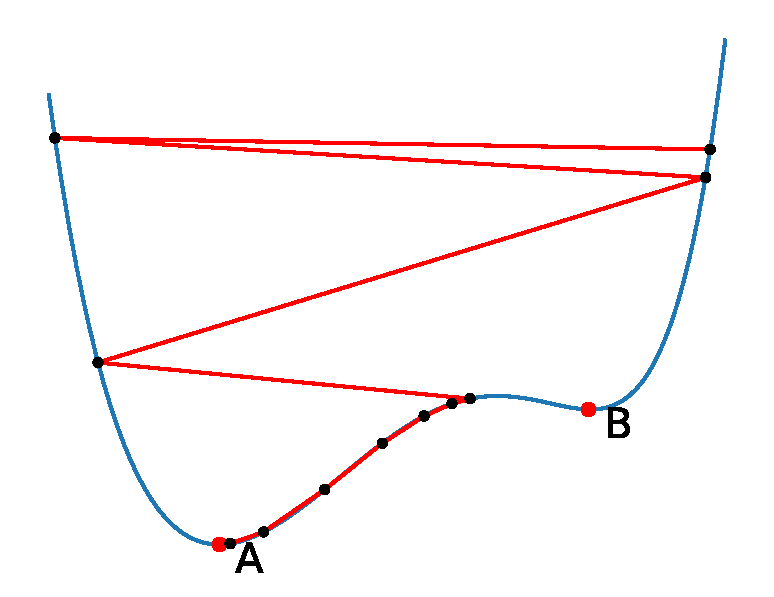
\includegraphics[width=\textwidth]{gradient_descent_large_lr}
        \caption{Gradient descent with a large learning rate.}
        \label{fig:gradient-descent-large}
    \end{subfigure}
    \caption{Gradient descent with different learning rates. Choosing the learning rate too small can lead to slow convergence and to being stuck in local minima. Choosing the learning rate too large can lead to \textit{overshooting} and to the algorithm diverging. Here, the algorithm still converges, but the large oscillations slow down the convergence.}
    \label{fig:gradient-descent}
\end{figure}
If we imagine the function $f(\bm{x})$ as a landscape, the goal of gradient descent is to find the lowest point of the landscape.
To do this, the algorithm starts at some point $\bm{x}_0$ and in each iteration, it takes a step in the direction of the steepest descent. 
The size of the step is determined by the \textit{learning rate} $\eta$.
Choosing an appropriate learning rate is crucial for the algorithm to converge.
Figure \ref{fig:gradient-descent} shows gradient descent with different learning rates and the resulting paths through the landscape.
\\
\\
As is known from multivariable calculus, the direction of the steepest descent of a function $f(\bm{x})$ is given by the negative gradient $\nabla f(\bm{x})$.
We can therefore update the parameters $\bm{x}$ in each iteration by:
\begin{equation}
    \bm{x}_{n+1} = \bm{x}_n - \eta \nabla f(\bm{x}_n) \text{.}
    \label{eq:gradient-descent}
\end{equation}
After a sufficient number of iterations, the algorithm will converge to a local minimum of the function. 
In the region around the minimum, the gradient is close to zero and the algorithm will not change the parameters significantly anymore.
We therefore define a threshold $\epsilon$ and stop the algorithm if the norm of the gradient falls below this threshold. 
The gradient descent algorithm is summarized in algorithm \ref{alg:gradient-descent}.
\begin{algorithm}
    \caption{Gradient Descent}
    \label{alg:gradient-descent}
    \begin{algorithmic}[1]
        \renewcommand{\algorithmicensure}{\textbf{Output:}}
        \Require
            \Statex $f(\bm{x})$: Function to minimize
            \Statex $\eta$: Learning rate
            \Statex $\epsilon$: Threshold
            \Statex $\bm{x}_0$: Initial parameters
        \Ensure $\bm{x^*}=\arg\min f(\bm{x})$: Parameters that minimize $f(\bm{x})$
        \output{$\bm{x\star}=\arg\min f(\bm{x})$: Parameters that minimize $f(\bm{x})$}
        \Statex
        \State $\bm{x} \gets \bm{x}_0$ \Comment{Initialize parameters}
        \While{$\norm{\nabla f(\bm{x}_n)} > \epsilon$} \Comment{Until convergence}
            \State $\bm{x} \gets \bm{x} - \eta \nabla f(\bm{x})$ \Comment{Update parameters}
        \EndWhile
        \State \Return $\bm{x}$ \Comment{Return parameters}
    \end{algorithmic}
\end{algorithm}

Going back to neural networks, the function that we want to minimize is the loss function $\lambda(\bm{y}, \bm{\hat{y}})$. 
As the loss function depends on the network's output $\bm{y}$, which in turn depends on the network's parameters $\bm{w}$ and $\bm{b}$, the loss function is a function of the network's parameters $\lambda(\bm{w}, \bm{b})$. 
\\
\\
For single layer networks, the calculation of the gradients is straightforward. 
For multi-layer networks however, the loss function depends on the parameters of earlier layers in a non-trivial way. 
The next section will outline an algorithm, that allows the efficient calculation of the gradients of multi-layer networks.

\subsection{The Backpropagation Algorithm}
\label{subsec:backprop}
% Goodfellow Ch. 6.5
% Aggarwal Ch. 1.3
% Jonas BA
The calculation of the gradients is the most computationally expensive part of training a neural network. The invention of the \textit{backpropagation} algorithm by Rumelhart et al. in 1986~\cite{rumelhart_learning_1986} was a major breakthrough in the field of neural networks, as it allowed very efficient gradient calculation and thus enabled the training of large neural networks. 
\\
The idea behind backpropagation is to propagate the error back through the network after each forward-propagation step using \textit{local gradients} $\delta$.
During the forward-propagation step, the activations of each layer are stored in memory and used to calculate the derivatives need for the backpropagation step.
This is a form of \textit{automatic differentiation}~\cite{adams_backprop_autodiff_nodate,rall_autodiff_1981} and allows the calculation of the gradients with the same time complexity as the forward-propagation step.
This is sometimes called the \textit{cheap gradient principle}~\cite{griewank_derivatives_2008}. The following mathematical derivation of the backpropagation algorithm is based on~\cite[chapter 4.4]{haykin_neural_1998} as well as~\cite[chapter 6.5]{goodfellow_deep_2016}.
\\
\\
To calculate the update of a weight $w_{ij}^{[K]}$, we have to calculate the derivative of the loss function $\lambda$ with respect to the weight $w_{ij}^{[K]}$:
\begin{equation}
    \Delta w_{ij}^{[K]} = \eta \cdot \frac{\partial \lambda}{\partial w_{ij}^{[K]}} \text{.}
    \label{eq:weight-derivative} 
\end{equation}
This derivative can be evaluated using the chain rule:
\begin{equation}
    \frac{\partial \lambda}{\partial w_{ij}^{[K]}} = \frac{\partial \lambda}{\partial a_i^{[K]}} \frac{\partial a_i^{[K]}}{\partial z_i^{[K]}} \frac{\partial z_i^{[K]}}{\partial w_{ij}^{[K]}} = \delta_i^{[K]} a_j^{[K-1]} 
    \label{eq:chain-rule}
\end{equation}
where we used equation \ref{eq:pre-activation-vector} to simplify the last derivative and defined the local gradient $\delta_j^{[K]}$ as:
\begin{equation}
    \delta_i^{[K]} = \frac{\partial \lambda}{\partial a_i^{[K]}} \frac{\partial a_i^{[K]}}{\partial z_i^{[K]}} \text{.}
    \label{eq:local-gradient}
\end{equation}
Let's take a closer look at the local gradient $\delta_i^{[K]}$.
The second factor in equation \ref{eq:local-gradient} is the derivative of the activation function $\phi$ with respect to the pre-activation value $z_i^{[K]}$.
This term is straightforward to calculate. 
Remembering that the activation function is applied element-wise, using equation \ref{eq:activation-vector} we get:
\begin{equation}
    \frac{\partial a_i^{[K]}}{\partial z_i^{[K]}} = \frac{\partial \phi(z_i^{[K]})}{\partial z_i^{[K]}} = \phi'(z_i^{[K]}) \text{.}
    \label{eq:activation-derivative}
\end{equation}
The first factor in equation \ref{eq:local-gradient} is the derivative of the loss function $\lambda$ with respect to the activation $a_i^{[K]}$.
If layer $K$ is the output layer, this derivative is simply the derivative of the loss function with respect to the output value $y_i$:
\begin{equation}
    \frac{\partial \lambda}{\partial a_i^{[K]}} = \frac{\partial \lambda}{\partial y_i} \text{.}
    \label{eq:loss-derivative-output}
\end{equation}
If layer $K$ is not the output layer, the derivative is slightly more complicated.
We can use the chain rule trick again, re-introducing the activation values $a_n^{[K+1]}$ of the next layer, which all depend on $a_i^{[K]}$:
\begin{equation}
    \frac{\partial \lambda}{\partial a_i^{[K]}} = \sum_{n=1}^{m_{K+1}} \frac{\partial \lambda}{\partial a_n^{[K+1]}} \frac{\partial a_n^{[K+1]}}{\partial a_i^{[K]}} = \sum_{n=1}^{m_{K+1}} \frac{\partial \lambda}{\partial a_n^{[K+1]}} \frac{\partial a_n^{[K+1]}}{\partial z_n^{[K+1]}} \frac{\partial z_n^{[K+1]}}{\partial a_i^{[K]}} \text{.}
    \label{eq:loss-derivative-hidden}
\end{equation}
Similar to equation \ref{eq:chain-rule}, we can use equation \ref{eq:pre-activation-vector} to simplify the last derivative and identify the local gradients $\delta_n^{[K+1]}$: 
\begin{equation}
    \frac{\partial \lambda}{\partial a_i^{[K]}} = \sum_{n=1}^{m_{K+1}} \delta_n^{[K+1]} w_{ni}^{[K+1]} \text{.}
    \label{eq:loss-derivative-hidden-simplified}
\end{equation}
Plugging equations \ref{eq:activation-derivative} and \ref{eq:loss-derivative-output} or \ref{eq:loss-derivative-hidden-simplified} back into equation \ref{eq:local-gradient} yields the final form of the local gradient:
\begin{equation}
    \delta_i^{[K]} = \phi'(z_i^{[K]}) \cdot \begin{cases}
         \frac{\partial \lambda}{\partial y_i} & \text{if layer } K \text{ is the output layer} \\
         \sum_{n=1}^{m_{K+1}} \delta_n^{[K+1]} w_{ni}^{[K+1]} & \text{otherwise} \text{.}
    \end{cases}
    \label{eq:local-gradient-final}
\end{equation}
This equation can be applied recursively to calculate the local gradients of all layers from the output layer to the input layer.
The weight update $\Delta w_{ij}^{[K]}$ can then be calculated using equation \ref{eq:weight-derivative} and \ref{eq:local-gradient-final}:
\begin{equation}
    \Delta w_{ij}^{[K]} = \eta \cdot \delta_i^{[K]} a_j^{[K-1]} \text{.}
    \label{eq:weight-update}
\end{equation}
When introducing the backpropagation algorithm, I summarized it as a method of \textit{propagating the error back through the network}.
The recursive usage of equation \ref{eq:local-gradient-final} is exactly that: We start at the output layer and calculate the local gradients of all nodes in the output layer using equation \ref{eq:local-gradient-final}.
Then we use these local gradients to calculate the local gradients of the previous layer using equation \ref{eq:local-gradient-final} again and so on until we reach the input layer. 
Note that we need to store the activations of each layer in memory during the \textit{forward-pass} to calculate the updates during the \textit{backward-pass} as mentioned in the beginning of this section.
\\
\\
The derivations for the bias updates are analogous to the weight updates and are therefore omitted here. 
The only difference is that the last term in equation \ref{eq:chain-rule} is replaced by $1$ as the bias is not connected to any previous layer.
The algorithm for a whole training step (i.e. one forward-pass and one backward-pass) is summarized in algorithm \ref{alg:backpropagation}.
\begin{algorithm}
    \caption{One training step of a neural network: Forward- and Backpropagation}
    \label{alg:backpropagation}
    \begin{algorithmic}[1]
        \renewcommand{\algorithmicensure}{\textbf{Output:}}
        \Require
            \Statex $\bm{x}$: Input vector
            \Statex $\bm{\hat{y}}$: Target output vector
            \Statex $\bm{w}$: Weight array containing all weight matrices $\bm{w}^{[K]}$
            \Statex $\bm{b}$: Bias array containing all bias vectors $\bm{b}^{[K]}$
            \Statex $\lambda$: Loss function
            \Statex $\phi$: Activation function
            \Statex $\eta$: Learning rate
        \Ensure Updates the weights $\bm{w}$ and biases $\bm{b}$ of the network inplace.
        \Statex
        \State $\bm{a}^{[0]} \gets \bm{x}$ \Comment{Initialize activations}
        \For{$K = 1, \dots, L$} \Comment{Forward-pass}
            \State $\bm{z}^{[K]} \gets \bm{w}^{[K]} \bm{a}^{[K-1]} + \bm{b}^{[K]}$ \Comment{Calculate pre-activations}
            \State $\bm{a}^{[K]} \gets \phi(\bm{z}^{[K]})$ \Comment{Calculate activations}
        \EndFor
        \State $\delta^{[L]} \gets \phi'(\bm{z}^{[L]}) \cdot \frac{\partial \lambda(\bm{a}^{[L]}, \bm{\hat{y}})}{\partial \bm{a}^{[L]}}$ \Comment{Initialize local gradients}
        \For{$K = L, \dots, 1$} \Comment{Backward-pass}
            \State $\Delta \bm{w}^{[K]} \gets \eta \cdot \delta^{[K]} \bm{a}^{[K-1]}$ \Comment{Calculate weight updates}
            \State $\Delta \bm{b}^{[K]} \gets \eta \cdot \delta^{[K]}$ \Comment{Calculate bias updates}
            \State $\delta^{[K-1]} \gets \phi'(\bm{z}^{[K-1]}) \cdot \bm{w}^{[K]T} \delta^{[K]}$ \Comment{Calculate local gradients}
        \EndFor
        \State $\bm{w} \gets \bm{w} - \Delta \bm{w}$ \Comment{Update weights}
        \State $\bm{b} \gets \bm{b} - \Delta \bm{b}$ \Comment{Update biases}
    \end{algorithmic}
\end{algorithm}

\subsection{Summary}
\label{subsec:nn-summary}
In this chapter, the foundations of neural networks were outlined.
Section~\ref{subsec:single-neuron} started by defining the building blocks of neural networks: The \textit{nodes}.
Section~\ref{subsec:forward-propagation} combined \textit{Layers} of these nodes into a \textit{fully connected neural network}.
The specific \textit{architecture} of the network, that is the number of layers, the number of nodes per layer and the \textit{activation functions}, depends on the problem that is being solved.
Later, we will see that in our case of Deep-Q-Learning, the size of the \textit{input vector} is determined by the number of cells that are visible to the agent and the size of the \textit{output vector} is determined by the number of possible actions that the agent can take.
\\
\\
On this basis, the \textit{forward-propagation} step could be analyzed in detail and the significance of the activation function was explained.
Next, section~\ref{subsec:loss-functions} introduced the \textit{loss function} as a measure of the network's error and the \textit{gradient descent} algorithm was outlined as a method to minimize this error.
Finally, the \textit{backpropagation} algorithm treated in section~\ref{subsec:backprop} provides a way to efficiently compute the gradients needed for gradient descent and enables the \textit{training} of large neural networks.
The whole process of forward-propagation, followed by backpropagation and network parameter updates is summarized in pseudocode in algorithm~\ref{alg:backpropagation}.





\chapter{Deep Q-Learning}
\label{ch:dql}


\section{Reinforcement Learning}
Out of the three main branches of machine learning, \textit{supervised learning}, \textit{unsupervised learning} and \textit{reinforcement learning}, reinforcement learning is the most similar to the way humans learn. 
\\
While supervised learning is based on the idea of learning from examples and unsupervised learning is concerned with finding patterns in data \cite{ibm_machine_learning}, reinforcement learning is based on the idea of learning from experience \cite[chapter 1.1]{sutton_reinforcement_nodate}.
In reinforcement learning, the learning agent is not told what action to take, but instead has to learn which actions lead to a desired outcome by trial and error. 
\\
This framework has led to many successes over the last decades, including computer programs that beat the world's best players in board games like chess, Go, backgammon \cite{silver_mastering_2016,silver_mastering_2017,tesauro_temporal_1995} or even in video games like Atari games \cite{mnih_playing_2013} and Dota 2 \cite{openai_dota_2019}, as well as teaching robots how to walk and handle objects \cite{kober_reinforcement_2013,openai_learning_2019}.
\textcolor{red}{TODO: Add OpenAI $Q^*$ here?}

\subsection{Overview}
In a reinforcement learning scenario, the \textit{agent} observes some information about the \textit{environment}, called the \textit{state} of the environment.
It then uses its \textit{policy} to map the state to an \textit{action} that it takes in the environment.
As a reaction, the environment returns a \textit{reward} to the agent and transitions to a new state \cite{openai_spinning_up_rl_intro}
\\
During the learning process, the agent tries to find a policy that maximizes the total reward that it receives from the environment. Depending on the type of problem, the agent can either try to maximize the reward in the short term or in the long term.
\\
\\
The following sections will refine these concepts and introduce the formalism of reinforcement learning.

\subsection{Notation}
\label{subsec:notation}
Before diving into the details of reinforcement learning, I will introduce the notation that will be used throughout the following sections. It is mostly identical to the notation used in \cite{sutton_reinforcement_nodate}. Some of these definitions might seem a bit abstract at first, but they will become clearer in the following sections, where they are introduced and explained one by one.

\begin{itemize}
    \item $s_t$: The state of the environment at time step $t$.
    \item $a_t$: The action taken by the agent at time step $t$, based on the state $s_t$.
    \item $r_t$: The reward returned by the environment at time step $t$, based on the state $s_t$, action $a_t$ and the new state $s_{t+1}$.
    \item $\pi$: The policy of the agent, mapping states to actions.
    \item $\pi(a|s)$: The probability of the agent taking action $a$ in state $s$.
    \item $p(s_{t+1} | s_t, a_t)$: The probability of the environment transitioning to state $s_{t+1}$ after the agent takes action $a_t$ in state $s_t$.
    \item $\tau$: A trajectory, i.e. a sequence of states, actions and rewards $(s_0, a_0, r_0, s_1, a_1, r_1, \dots)$.
    \item $G_t$: The return at time step $t$, i.e. the total discounted reward from time step $t$ onwards.
    \item $\gamma$: The discount factor, determining how much future rewards are worth compared to immediate rewards.
    \item $v_\pi(s)$: The value of state $s$ under policy $\pi$, i.e. the expected return when starting in state $s$ and following policy $\pi$.
    \item $q_\pi(s, a)$: The value of taking action $a$ in state $s$ under policy $\pi$, i.e. the expected return when starting in state $s$, taking action $a$ and then following policy $\pi$.
    \item $\pi_*, v_*, q_*$: The optimal policy, value function and action-value function respectively.
\end{itemize}


\subsection{Important Concepts}

\subsubsection{Markov Decision Processes}
\begin{figure}[h]
    \centering
    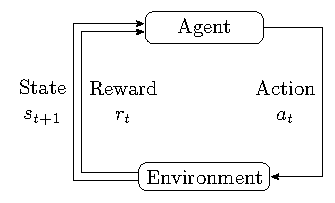
\includegraphics[width=0.5\textwidth]{agent_env_interface.pdf}
    \caption{The agent-environment interface in a Markov decision process as defined in \cite[chapter 3.1]{sutton_reinforcement_nodate}. The agent observes the state $s_t$ of the environment and takes an action $a_t$. The environment transitions to a new state $s_{t+1}$ and returns a reward $r_{t}$ to the agent.}
    \label{fig:agent-env-interface}
\end{figure}
Markov decision processes (MDPs) are a mathematical framework for modeling decision-making in situations where outcomes are partly random and only partly under the control of the agent \cite[chapter 3]{sutton_reinforcement_nodate}. In an MDP, the agent's actions influence not only the immediate reward, but also the next state of the environment and therefore all future rewards.
They are a powerful abstraction that can be used to model a wide range of problems, from simple board games to complex real-world scenarios. \\
MDPs can be seen as a generalization of discrete-time \textit{Markov chains}.
Markov chains are a special case of \textit{stochastic processes}, where the next state of the system is determined only by the current state and not by any previous states.
This property is called the \textit{Markov property} and can be expressed mathematically as \cite{serfozo_markov_2009}:
\begin{equation}
    p(s_{t+1} | s_1, \dots, s_t) = p(s_{t+1} | s_t) = p_{ss'} \text{.}
    \label{eq:markov-property}
\end{equation}
The probability $P$ of transitioning to state $s_{t+1}$ from state $s_t$ is independent of the previous states $s_1, \dots, s_{t-1}$ and only depends on the current state $s_t$.
It is intuitive that the state trajectories in a reinforcement learning scenario should always satisfy this property, as it allows the agent to make decisions based on the current state without having to consider the whole history of states that led to the current state. 
\\
\\
MDPs slightly modify the definition of Markov chains by introducing the notion of actions and rewards.
As outlined in the previous section, the agent interacts with the environment by taking actions $a_i$ based on the current state of the environment $s_i$ and receives rewards $r_i$ from the environment in return.
This \textit{agent-environment interface} is illustrated in figure \ref{fig:agent-env-interface}.
A \textit{trajectory} $\tau$ in an MDP is a sequence of states, actions and rewards \cite[48]{sutton_reinforcement_nodate}:
\begin{equation}
    \tau = (s_0, a_0, r_0, s_1, a_1, r_1, s_2, \dots) \text{.}
    \label{eq:trajectory}
\end{equation}
The transition probability now depends on the action $a_t$ that the agent takes in state $s_t$:
\begin{align}
    p: \mathcal{S} \times \mathcal{R} \times \mathcal{S} \times \mathcal{A} &\rightarrow [0, 1] \nonumber \\
    s_{t+1}, r_t, s_t, a_t &\mapsto p(s_{t+1}, r_t | s_t, a_t) \text{,}
    \label{eq:transition-probability}
\end{align}
where $\mathcal{S}$ denotes the set of all possible states and $\mathcal{A}$ denotes the set of all possible actions.\\
This probability function completely determines the dynamics of the reinforcement learning environment. Environments can be entirely deterministic or entirely stochastic, or anything in between. The four-argument transition probability, if known, can of course be used to calculate other properties of the environment, such as the three-argument state-transition probability \cite[49]{sutton_reinforcement_nodate}:
\begin{align}
    p: \mathcal{S} \times \mathcal{S} \times \mathcal{A} &\rightarrow [0, 1] \nonumber \\
    s_{t+1}, s_t, a_t &\mapsto p(s_{t+1} | s_t, a_t) = \sum_{r_t \in \mathcal{R}} p(s_{t+1}, r_t | s_t, a_t) \text{.}
    \label{eq:state-transition-probability}
\end{align}
where $\mathcal{R}$ denotes the set of all possible rewards.\\
Furthermore, knowing the four-argument transition probability of an environment allows us to create a simulation of the environment, which can be used to test reinforcement learning algorithms. This is a very useful property, as it allows us to test reinforcement learning algorithms in a controlled environment before deploying them in the real world.\\

\subsubsection{Reward}
After each time step $t$, the agent receives a reward $r_t$ from the environment. The reward is a scalar value that indicates how good or bad the action $a_t$ that the agent took in state $s_t$ was \cite[53]{sutton_reinforcement_nodate}. Rewards are the \enquote{trainer's} way of telling the agent what it should achieve. In order to use the full potential of reinforcement learning, rewards should be chosen carefully. The reward signal should not tell the agent \textit{how} to achieve the goal, but only \textit{what} the goal is. The agent should then be able to figure out the best way to achieve the goal by itself \cite[ch. 3.2]{sutton_reinforcement_nodate}. For example, if the goal is to teach a robot to walk, the agent should receive a reward for moving forward while maintaining a certain balance, but not for moving its legs in a certain way.
\\
In order to be able to learn from these rewards, not just the immediate reward $r_t$ should be taken into account, but also the rewards that the agent will receive in the future. This is done by introducing the notion of \textit{return}. The return $G_t$ is a measure of the cumulative reward that the agent will receive from time step $t$ onwards \cite[ch. 3.3]{sutton_reinforcement_nodate}. The simplest form of return is just the sum of all future rewards:
\begin{equation}
    G_t = r_t + r_{t+1} + r_{t+2} + \dots + r_{T} = \sum_{i=t}^{T} r_{i} \text{,}
    \label{eq:return}
\end{equation}
where $T$ is the final time step in the current \textit{episode}. Episodic tasks are task where a \textit{terminal state} $s_T$ can be reached, after which the episode ends. Examples are board games like chess or Go, where the game ends after one player wins. In contrast, for \textit{continuing tasks}, as is the case for the environment that we will consider in this thesis, there is no terminal state and $T=\infty$. In this case, it's useful to introduce a \textit{discounted} return \cite[ch. 3.3]{sutton_reinforcement_nodate}:
\begin{equation}
    G_t = r_t + \gamma r_{t+1} + \gamma^2 r_{t+2} + \dots = \sum_{i=t}^{\infty} \gamma^{i-t} r_{i} \text{.}
    \label{eq:discounted-return}
\end{equation}
The \textit{discount factor} $\gamma$ determines how much immediate rewards should be valued compared to future rewards. A discount factor of $\gamma=0$ means that only the immediate reward is taken into account, while a discount factor of $\gamma=1$ would value all future rewards equally. \\
The discounted reward formula can be rewritten recursively as \cite[55]{sutton_reinforcement_nodate}:
\begin{align}
    G_t &= r_t + \gamma r_{t+1} + \gamma^2 r_{t+2} + \dots \nonumber \\
    &= r_t + \gamma (r_{t+1} + \gamma r_{t+2} + \dots) \nonumber \\
    &= r_t + \gamma G_{t+1} \text{.}
    \label{eq:discounted-return-recursive}
\end{align}
%%important later expected return claculation


\subsubsection{Policies and Value Functions}

\subsubsection{Optimality and Bellman Equations}

\subsection{Summary}

\subsection{Algorithms}



\section{Deep Q-Learning}